% Created by tikzDevice version 0.12 on 2019-04-30 12:38:12
% !TEX encoding = UTF-8 Unicode
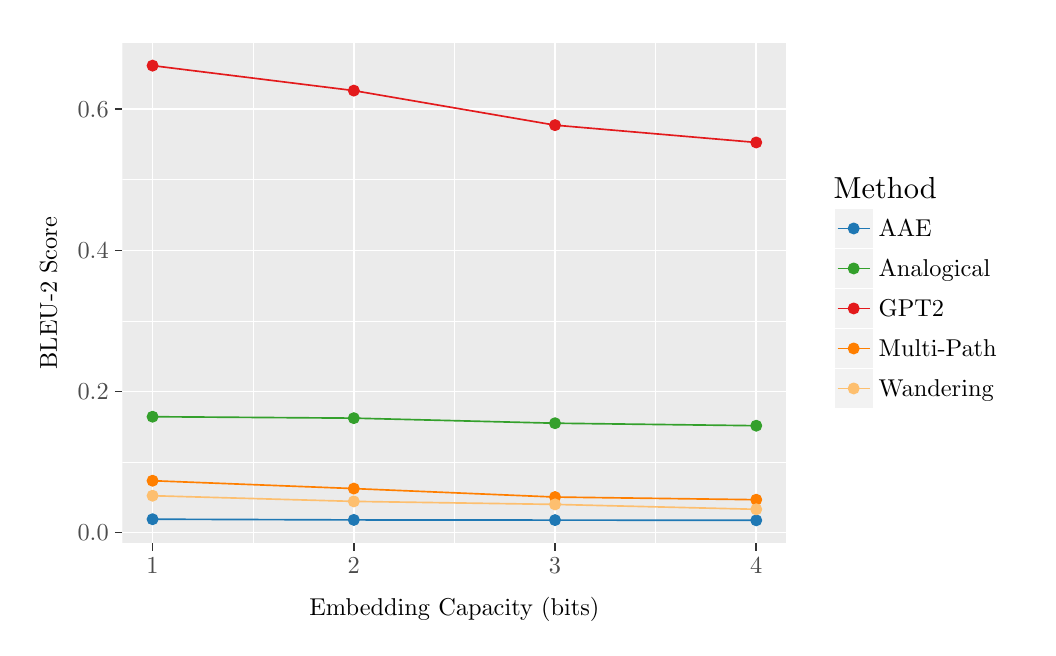
\begin{tikzpicture}[x=1pt,y=1pt]
\definecolor{fillColor}{RGB}{255,255,255}
\path[use as bounding box,fill=fillColor,fill opacity=0.00] (0,0) rectangle (361.35,216.81);
\begin{scope}
\path[clip] (  0.00,  0.00) rectangle (361.35,216.81);
\definecolor{drawColor}{RGB}{255,255,255}
\definecolor{fillColor}{RGB}{255,255,255}

\path[draw=drawColor,line width= 0.6pt,line join=round,line cap=round,fill=fillColor] (  0.00,  0.00) rectangle (361.35,216.81);
\end{scope}
\begin{scope}
\path[clip] ( 34.22, 30.57) rectangle (274.18,211.31);
\definecolor{fillColor}{gray}{0.92}

\path[fill=fillColor] ( 34.22, 30.57) rectangle (274.18,211.31);
\definecolor{drawColor}{RGB}{255,255,255}

\path[draw=drawColor,line width= 0.3pt,line join=round] ( 34.22, 59.86) --
	(274.18, 59.86);

\path[draw=drawColor,line width= 0.3pt,line join=round] ( 34.22,110.84) --
	(274.18,110.84);

\path[draw=drawColor,line width= 0.3pt,line join=round] ( 34.22,161.82) --
	(274.18,161.82);

\path[draw=drawColor,line width= 0.3pt,line join=round] ( 81.49, 30.57) --
	( 81.49,211.31);

\path[draw=drawColor,line width= 0.3pt,line join=round] (154.20, 30.57) --
	(154.20,211.31);

\path[draw=drawColor,line width= 0.3pt,line join=round] (226.92, 30.57) --
	(226.92,211.31);

\path[draw=drawColor,line width= 0.6pt,line join=round] ( 34.22, 34.36) --
	(274.18, 34.36);

\path[draw=drawColor,line width= 0.6pt,line join=round] ( 34.22, 85.35) --
	(274.18, 85.35);

\path[draw=drawColor,line width= 0.6pt,line join=round] ( 34.22,136.33) --
	(274.18,136.33);

\path[draw=drawColor,line width= 0.6pt,line join=round] ( 34.22,187.32) --
	(274.18,187.32);

\path[draw=drawColor,line width= 0.6pt,line join=round] ( 45.13, 30.57) --
	( 45.13,211.31);

\path[draw=drawColor,line width= 0.6pt,line join=round] (117.85, 30.57) --
	(117.85,211.31);

\path[draw=drawColor,line width= 0.6pt,line join=round] (190.56, 30.57) --
	(190.56,211.31);

\path[draw=drawColor,line width= 0.6pt,line join=round] (263.27, 30.57) --
	(263.27,211.31);
\definecolor{drawColor}{RGB}{31,120,180}

\path[draw=drawColor,line width= 0.6pt,line join=round] ( 45.13, 39.19) --
	(117.85, 38.94) --
	(190.56, 38.87) --
	(263.27, 38.79);
\definecolor{drawColor}{RGB}{52,160,44}

\path[draw=drawColor,line width= 0.6pt,line join=round] ( 45.13, 76.23) --
	(117.85, 75.71) --
	(190.56, 73.88) --
	(263.27, 72.98);
\definecolor{drawColor}{RGB}{227,26,28}

\path[draw=drawColor,line width= 0.6pt,line join=round] ( 45.13,203.09) --
	(117.85,194.07) --
	(190.56,181.58) --
	(263.27,175.33);
\definecolor{drawColor}{RGB}{255,127,0}

\path[draw=drawColor,line width= 0.6pt,line join=round] ( 45.13, 53.10) --
	(117.85, 50.26) --
	(190.56, 47.20) --
	(263.27, 46.24);
\definecolor{drawColor}{RGB}{253,191,111}

\path[draw=drawColor,line width= 0.6pt,line join=round] ( 45.13, 47.68) --
	(117.85, 45.63) --
	(190.56, 44.54) --
	(263.27, 42.77);
\definecolor{drawColor}{RGB}{31,120,180}
\definecolor{fillColor}{RGB}{31,120,180}

\path[draw=drawColor,line width= 0.4pt,line join=round,line cap=round,fill=fillColor] ( 45.13, 39.19) circle (  1.96);

\path[draw=drawColor,line width= 0.4pt,line join=round,line cap=round,fill=fillColor] (117.85, 38.94) circle (  1.96);

\path[draw=drawColor,line width= 0.4pt,line join=round,line cap=round,fill=fillColor] (190.56, 38.87) circle (  1.96);

\path[draw=drawColor,line width= 0.4pt,line join=round,line cap=round,fill=fillColor] (263.27, 38.79) circle (  1.96);
\definecolor{drawColor}{RGB}{227,26,28}
\definecolor{fillColor}{RGB}{227,26,28}

\path[draw=drawColor,line width= 0.4pt,line join=round,line cap=round,fill=fillColor] ( 45.13,203.09) circle (  1.96);

\path[draw=drawColor,line width= 0.4pt,line join=round,line cap=round,fill=fillColor] (117.85,194.07) circle (  1.96);

\path[draw=drawColor,line width= 0.4pt,line join=round,line cap=round,fill=fillColor] (190.56,181.58) circle (  1.96);

\path[draw=drawColor,line width= 0.4pt,line join=round,line cap=round,fill=fillColor] (263.27,175.33) circle (  1.96);
\definecolor{drawColor}{RGB}{255,127,0}
\definecolor{fillColor}{RGB}{255,127,0}

\path[draw=drawColor,line width= 0.4pt,line join=round,line cap=round,fill=fillColor] ( 45.13, 53.10) circle (  1.96);

\path[draw=drawColor,line width= 0.4pt,line join=round,line cap=round,fill=fillColor] (117.85, 50.26) circle (  1.96);

\path[draw=drawColor,line width= 0.4pt,line join=round,line cap=round,fill=fillColor] (190.56, 47.20) circle (  1.96);

\path[draw=drawColor,line width= 0.4pt,line join=round,line cap=round,fill=fillColor] (263.27, 46.24) circle (  1.96);
\definecolor{drawColor}{RGB}{52,160,44}
\definecolor{fillColor}{RGB}{52,160,44}

\path[draw=drawColor,line width= 0.4pt,line join=round,line cap=round,fill=fillColor] ( 45.13, 76.23) circle (  1.96);

\path[draw=drawColor,line width= 0.4pt,line join=round,line cap=round,fill=fillColor] (117.85, 75.71) circle (  1.96);

\path[draw=drawColor,line width= 0.4pt,line join=round,line cap=round,fill=fillColor] (190.56, 73.88) circle (  1.96);

\path[draw=drawColor,line width= 0.4pt,line join=round,line cap=round,fill=fillColor] (263.27, 72.98) circle (  1.96);
\definecolor{drawColor}{RGB}{253,191,111}
\definecolor{fillColor}{RGB}{253,191,111}

\path[draw=drawColor,line width= 0.4pt,line join=round,line cap=round,fill=fillColor] ( 45.13, 47.68) circle (  1.96);

\path[draw=drawColor,line width= 0.4pt,line join=round,line cap=round,fill=fillColor] (117.85, 45.63) circle (  1.96);

\path[draw=drawColor,line width= 0.4pt,line join=round,line cap=round,fill=fillColor] (190.56, 44.54) circle (  1.96);

\path[draw=drawColor,line width= 0.4pt,line join=round,line cap=round,fill=fillColor] (263.27, 42.77) circle (  1.96);
\end{scope}
\begin{scope}
\path[clip] (  0.00,  0.00) rectangle (361.35,216.81);
\definecolor{drawColor}{gray}{0.30}

\node[text=drawColor,anchor=base east,inner sep=0pt, outer sep=0pt, scale=  0.88] at ( 29.27, 31.33) {0.0};

\node[text=drawColor,anchor=base east,inner sep=0pt, outer sep=0pt, scale=  0.88] at ( 29.27, 82.32) {0.2};

\node[text=drawColor,anchor=base east,inner sep=0pt, outer sep=0pt, scale=  0.88] at ( 29.27,133.30) {0.4};

\node[text=drawColor,anchor=base east,inner sep=0pt, outer sep=0pt, scale=  0.88] at ( 29.27,184.29) {0.6};
\end{scope}
\begin{scope}
\path[clip] (  0.00,  0.00) rectangle (361.35,216.81);
\definecolor{drawColor}{gray}{0.20}

\path[draw=drawColor,line width= 0.6pt,line join=round] ( 31.47, 34.36) --
	( 34.22, 34.36);

\path[draw=drawColor,line width= 0.6pt,line join=round] ( 31.47, 85.35) --
	( 34.22, 85.35);

\path[draw=drawColor,line width= 0.6pt,line join=round] ( 31.47,136.33) --
	( 34.22,136.33);

\path[draw=drawColor,line width= 0.6pt,line join=round] ( 31.47,187.32) --
	( 34.22,187.32);
\end{scope}
\begin{scope}
\path[clip] (  0.00,  0.00) rectangle (361.35,216.81);
\definecolor{drawColor}{gray}{0.20}

\path[draw=drawColor,line width= 0.6pt,line join=round] ( 45.13, 27.82) --
	( 45.13, 30.57);

\path[draw=drawColor,line width= 0.6pt,line join=round] (117.85, 27.82) --
	(117.85, 30.57);

\path[draw=drawColor,line width= 0.6pt,line join=round] (190.56, 27.82) --
	(190.56, 30.57);

\path[draw=drawColor,line width= 0.6pt,line join=round] (263.27, 27.82) --
	(263.27, 30.57);
\end{scope}
\begin{scope}
\path[clip] (  0.00,  0.00) rectangle (361.35,216.81);
\definecolor{drawColor}{gray}{0.30}

\node[text=drawColor,anchor=base,inner sep=0pt, outer sep=0pt, scale=  0.88] at ( 45.13, 19.56) {1};

\node[text=drawColor,anchor=base,inner sep=0pt, outer sep=0pt, scale=  0.88] at (117.85, 19.56) {2};

\node[text=drawColor,anchor=base,inner sep=0pt, outer sep=0pt, scale=  0.88] at (190.56, 19.56) {3};

\node[text=drawColor,anchor=base,inner sep=0pt, outer sep=0pt, scale=  0.88] at (263.27, 19.56) {4};
\end{scope}
\begin{scope}
\path[clip] (  0.00,  0.00) rectangle (361.35,216.81);
\definecolor{drawColor}{RGB}{0,0,0}

\node[text=drawColor,anchor=base,inner sep=0pt, outer sep=0pt, scale=  0.88] at (154.20,  4.25) {Embedding Capacity (bits)};
\end{scope}
\begin{scope}
\path[clip] (  0.00,  0.00) rectangle (361.35,216.81);
\definecolor{drawColor}{RGB}{0,0,0}

\node[text=drawColor,rotate= 90.00,anchor=base,inner sep=0pt, outer sep=0pt, scale=  0.88] at ( 10.59,120.94) {BLEU-2 Score};
\end{scope}
\begin{scope}
\path[clip] (  0.00,  0.00) rectangle (361.35,216.81);
\definecolor{fillColor}{RGB}{255,255,255}

\path[fill=fillColor] (285.56, 73.52) rectangle (355.85,168.36);
\end{scope}
\begin{scope}
\path[clip] (  0.00,  0.00) rectangle (361.35,216.81);
\definecolor{drawColor}{RGB}{0,0,0}

\node[text=drawColor,anchor=base west,inner sep=0pt, outer sep=0pt, scale=  1.10] at (291.25,155.09) {Method};
\end{scope}
\begin{scope}
\path[clip] (  0.00,  0.00) rectangle (361.35,216.81);
\definecolor{drawColor}{RGB}{255,255,255}
\definecolor{fillColor}{gray}{0.95}

\path[draw=drawColor,line width= 0.6pt,line join=round,line cap=round,fill=fillColor] (291.25,137.03) rectangle (305.71,151.48);
\end{scope}
\begin{scope}
\path[clip] (  0.00,  0.00) rectangle (361.35,216.81);
\definecolor{drawColor}{RGB}{31,120,180}

\path[draw=drawColor,line width= 0.6pt,line join=round] (292.70,144.25) -- (304.26,144.25);
\end{scope}
\begin{scope}
\path[clip] (  0.00,  0.00) rectangle (361.35,216.81);
\definecolor{drawColor}{RGB}{31,120,180}
\definecolor{fillColor}{RGB}{31,120,180}

\path[draw=drawColor,line width= 0.4pt,line join=round,line cap=round,fill=fillColor] (298.48,144.25) circle (  1.96);
\end{scope}
\begin{scope}
\path[clip] (  0.00,  0.00) rectangle (361.35,216.81);
\definecolor{drawColor}{RGB}{255,255,255}
\definecolor{fillColor}{gray}{0.95}

\path[draw=drawColor,line width= 0.6pt,line join=round,line cap=round,fill=fillColor] (291.25,122.57) rectangle (305.71,137.03);
\end{scope}
\begin{scope}
\path[clip] (  0.00,  0.00) rectangle (361.35,216.81);
\definecolor{drawColor}{RGB}{52,160,44}

\path[draw=drawColor,line width= 0.6pt,line join=round] (292.70,129.80) -- (304.26,129.80);
\end{scope}
\begin{scope}
\path[clip] (  0.00,  0.00) rectangle (361.35,216.81);
\definecolor{drawColor}{RGB}{52,160,44}
\definecolor{fillColor}{RGB}{52,160,44}

\path[draw=drawColor,line width= 0.4pt,line join=round,line cap=round,fill=fillColor] (298.48,129.80) circle (  1.96);
\end{scope}
\begin{scope}
\path[clip] (  0.00,  0.00) rectangle (361.35,216.81);
\definecolor{drawColor}{RGB}{255,255,255}
\definecolor{fillColor}{gray}{0.95}

\path[draw=drawColor,line width= 0.6pt,line join=round,line cap=round,fill=fillColor] (291.25,108.12) rectangle (305.71,122.57);
\end{scope}
\begin{scope}
\path[clip] (  0.00,  0.00) rectangle (361.35,216.81);
\definecolor{drawColor}{RGB}{227,26,28}

\path[draw=drawColor,line width= 0.6pt,line join=round] (292.70,115.35) -- (304.26,115.35);
\end{scope}
\begin{scope}
\path[clip] (  0.00,  0.00) rectangle (361.35,216.81);
\definecolor{drawColor}{RGB}{227,26,28}
\definecolor{fillColor}{RGB}{227,26,28}

\path[draw=drawColor,line width= 0.4pt,line join=round,line cap=round,fill=fillColor] (298.48,115.35) circle (  1.96);
\end{scope}
\begin{scope}
\path[clip] (  0.00,  0.00) rectangle (361.35,216.81);
\definecolor{drawColor}{RGB}{255,255,255}
\definecolor{fillColor}{gray}{0.95}

\path[draw=drawColor,line width= 0.6pt,line join=round,line cap=round,fill=fillColor] (291.25, 93.66) rectangle (305.71,108.12);
\end{scope}
\begin{scope}
\path[clip] (  0.00,  0.00) rectangle (361.35,216.81);
\definecolor{drawColor}{RGB}{255,127,0}

\path[draw=drawColor,line width= 0.6pt,line join=round] (292.70,100.89) -- (304.26,100.89);
\end{scope}
\begin{scope}
\path[clip] (  0.00,  0.00) rectangle (361.35,216.81);
\definecolor{drawColor}{RGB}{255,127,0}
\definecolor{fillColor}{RGB}{255,127,0}

\path[draw=drawColor,line width= 0.4pt,line join=round,line cap=round,fill=fillColor] (298.48,100.89) circle (  1.96);
\end{scope}
\begin{scope}
\path[clip] (  0.00,  0.00) rectangle (361.35,216.81);
\definecolor{drawColor}{RGB}{255,255,255}
\definecolor{fillColor}{gray}{0.95}

\path[draw=drawColor,line width= 0.6pt,line join=round,line cap=round,fill=fillColor] (291.25, 79.21) rectangle (305.71, 93.66);
\end{scope}
\begin{scope}
\path[clip] (  0.00,  0.00) rectangle (361.35,216.81);
\definecolor{drawColor}{RGB}{253,191,111}

\path[draw=drawColor,line width= 0.6pt,line join=round] (292.70, 86.44) -- (304.26, 86.44);
\end{scope}
\begin{scope}
\path[clip] (  0.00,  0.00) rectangle (361.35,216.81);
\definecolor{drawColor}{RGB}{253,191,111}
\definecolor{fillColor}{RGB}{253,191,111}

\path[draw=drawColor,line width= 0.4pt,line join=round,line cap=round,fill=fillColor] (298.48, 86.44) circle (  1.96);
\end{scope}
\begin{scope}
\path[clip] (  0.00,  0.00) rectangle (361.35,216.81);
\definecolor{drawColor}{RGB}{0,0,0}

\node[text=drawColor,anchor=base west,inner sep=0pt, outer sep=0pt, scale=  0.88] at (307.51,141.22) {AAE};
\end{scope}
\begin{scope}
\path[clip] (  0.00,  0.00) rectangle (361.35,216.81);
\definecolor{drawColor}{RGB}{0,0,0}

\node[text=drawColor,anchor=base west,inner sep=0pt, outer sep=0pt, scale=  0.88] at (307.51,126.77) {Analogical};
\end{scope}
\begin{scope}
\path[clip] (  0.00,  0.00) rectangle (361.35,216.81);
\definecolor{drawColor}{RGB}{0,0,0}

\node[text=drawColor,anchor=base west,inner sep=0pt, outer sep=0pt, scale=  0.88] at (307.51,112.32) {GPT2};
\end{scope}
\begin{scope}
\path[clip] (  0.00,  0.00) rectangle (361.35,216.81);
\definecolor{drawColor}{RGB}{0,0,0}

\node[text=drawColor,anchor=base west,inner sep=0pt, outer sep=0pt, scale=  0.88] at (307.51, 97.86) {Multi-Path};
\end{scope}
\begin{scope}
\path[clip] (  0.00,  0.00) rectangle (361.35,216.81);
\definecolor{drawColor}{RGB}{0,0,0}

\node[text=drawColor,anchor=base west,inner sep=0pt, outer sep=0pt, scale=  0.88] at (307.51, 83.41) {Wandering};
\end{scope}
\end{tikzpicture}
